\section{Exercise 07: Brute Forcing Glassfish}

\subsection{What does https actually provide protection for?}
HTTPS provides website authentication, data privacy, and integrity by encrypting communications between client and server.
This protects against eavesdropping, tampering, and man-in-the-middle attacks.
HTTPS is crucial over insecure networks and protects sensitive information, even on networks prone to interference.

\subsection{Which username/password combination did you find?}
After i ran the glassfish i found the following username/password combination. Username: admin Password: sploit

\begin{figure}[H]
    \centering
    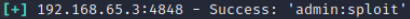
\includegraphics[width=0.7\linewidth]{pic/glassfish.png}
    \caption{Glassfish}
    \label{fig:glassfish}
\end{figure}

\subsection{Discuss which security relevant problems are we testing with a brute force attack?}
When we are testing with a brute force attack, we are looking for any poor configuration, easy to break / weak passwords and any lack of multi-factor-authentication (MFA)
within the system. We are also looking for any external ip addresses being allowed to sign in, and if they are allowing many login attempts or not.



\subsection{Discuss what would be your suggestions to the admin in order to address and mitigatethis issue?}
To strengthen the security against brute-force and dictionary attacks, the admin should implement account lockouts after repeated failed login attempts,
adding an email reset after a certain threshold, such as 5 attempts. This measure must be balanced to avoid denial-of-service (DOS) scenarios.
Enhancing password policies to require complex passwords will also reduce the efficacy of attacks. Also
implementing MFA provides an extra layer of security, even in the event of password leaks, as you also would need the authenticater device or key.
Access restrictions based on IP geolocation, or requiring a secure VPN connection for access, can further safeguard against unauthorized attempts to penetrate the organizations
systems.

\subsection{How is this attack type related to the internet of things, internet routers, and, e.g., virtual machines?}
Brute force attacks the target devices by repeatedly trying to gain access, making virtual machines, IoT devices, and internet routers vulnerable,
especially those with default or weak settings. IoT devices often come with factory-set passwords, known and rarely changed by users who may not have a lot of technical know how,
making them unsafe. Also routers with default passwords can be directly accessed for malicious purposes.
Virtual machines, if configured with standard passwords for convenience,
can be remotely exploited. Secure practices such as changing default credentials and employing complex passwords are important across all devices to
mimimiz the risk of brute force attacks.

\subsection{Do you know a way in which https could make the connection more secure against thiskind of attack?}
HTTPS enhances security by encrypting data during transmission, including login credentials.
It does not directly prevent brute force attacks but deters them by securing communication channels, stopping man-in-the-middle attempts,
and protecting against the leakage of passwords.
The encryption and server authentication aspects of HTTPS make it more challenging for attackers to intercept and use credentials for brute force attacks,
thereby mitigating the risk. also it ensures that passwords are not sent in plain text, which is important for preventing the leak of sensitive data.
